% !TEX root = ../main.tex

\section{Experimental Setup}
\label{sec:orgb44ba25}

We test multilabel learning using our proposed sigmoidF1 loss function on four datasets across different modalities, image and text. 
The datasets fit the FIMPUL characteristics. In particular, they are best modeled with full-instance learning as the entire image or the full text is predictive of the instance's labels. The next section and Table~\ref{table:datasets} describe our four datasets. The learning architecture (classification head attached to a pretrained net) is then described before addressing hyperparameter tuning and reproducibility remarks.

\subsection{Datasets}

Our first dataset comes from the vision domain and consists of movie posters and their genres (e.g., \emph{action}, \emph{comedy}).\footnote{Labels available at \url{https://tinyurl.com/y7ydyedu} and prescraped images from IMDB at \url{https://tinyurl.com/y7lfpvlx}.} The posters and labels have been extracted from IMDB and the dataset was previously used for per-class, post-training thresholding \citep{moviePosters} (see Section~\ref{sec:org2aceb9f}). The genre labels in this dataset are not mutually exclusive and of varying counts per movie. 

We use the newly created \emph{arXiv dataset}\footnote{Available at \url{https://www.kaggle.com/Cornell-University/arxiv}} with over 1.7 million open source articles and their metadata. Our experiments use the abstracts and categories that are suitably non-mutually exclusive and of varying counts per example. There is a longer history of using arXiv to create research datasets; the dataset we use is not to be confused with an earlier long document dataset that only features 11 classes~\citep{oldarXiv}, but was used in a recent long transformer publication~\cite{bigBird}. The limited number of labeled classes render the older dataset unsuitable for our experiments.  We write \textit{arXiv2020} for the subset of the \emph{arXiv dataset} that only contains documents published in 2020, given limited computing power. This results in around 26k documents.

To the best of our knowledge, ML-NET~\cite{multitaskLabel} is the state-of-the-art among \emph{fit-algorithm-to-data} methods for multilabel learning with unknown label count on text (the work does not differentiate full-instance and multi-instance learning, see Section~\ref{sec:org2aceb9f}). Among the three datasets used for benchmarking ML-NET, the cancerHallmark~\citep{cancerHallmarks}\footnote{Available at \url{https://github.com/sb895/Hallmarks-of-Cancer}} and chemicalExposure~\citep{chemExposure}\footnote{Available at \url{https://github.com/sb895/chemical-exposure-information-corpus}} datasets are of multi-instance multilabel nature: several expressions are annotated within each paper abstracts. The third dataset diagnosisCodes could not be obtained (neither from the authors of ML-NET nor of the original paper~\cite{diagnosisCode}). We treat cancerHallmarks and chemicalExposure as full-instance datasets by aggregating expression labels over each example, as was done for ML-NET.

\begin{table}
\caption{Descriptive statistics of our experimental datasets.}
\label{table:datasets}
\centering
% \begin{adjustbox}{max width=\textwidth}
\begin{tabular}{l rrrr}
\toprule
& & & Average & Number of \\
& Type & Classes & label count & examples \\
\midrule
moviePosters & image & 28 & 2.165 & 37,632\\
arXiv2020 & text & 155 & 1.888 & 26,558\\ 
chemExposure & text & 38 & 6.116 & 3,661\\
cancerHallmarks\hspace{-.7em}  & text & 33 & 3.501 & 1,582\\
\bottomrule
\end{tabular}
% \end{adjustbox}
\end{table}

\subsection{Learning framework}

The learning framework consists of two parts: a pretrained deep neural network and a classification head (see Figure \ref{fig:architecture}); the classification head is where we slot in alternative loss functions.

\begin{figure*}[htbp]
\centering
     \begin{subfigure}{0.6\linewidth}
         \centering
         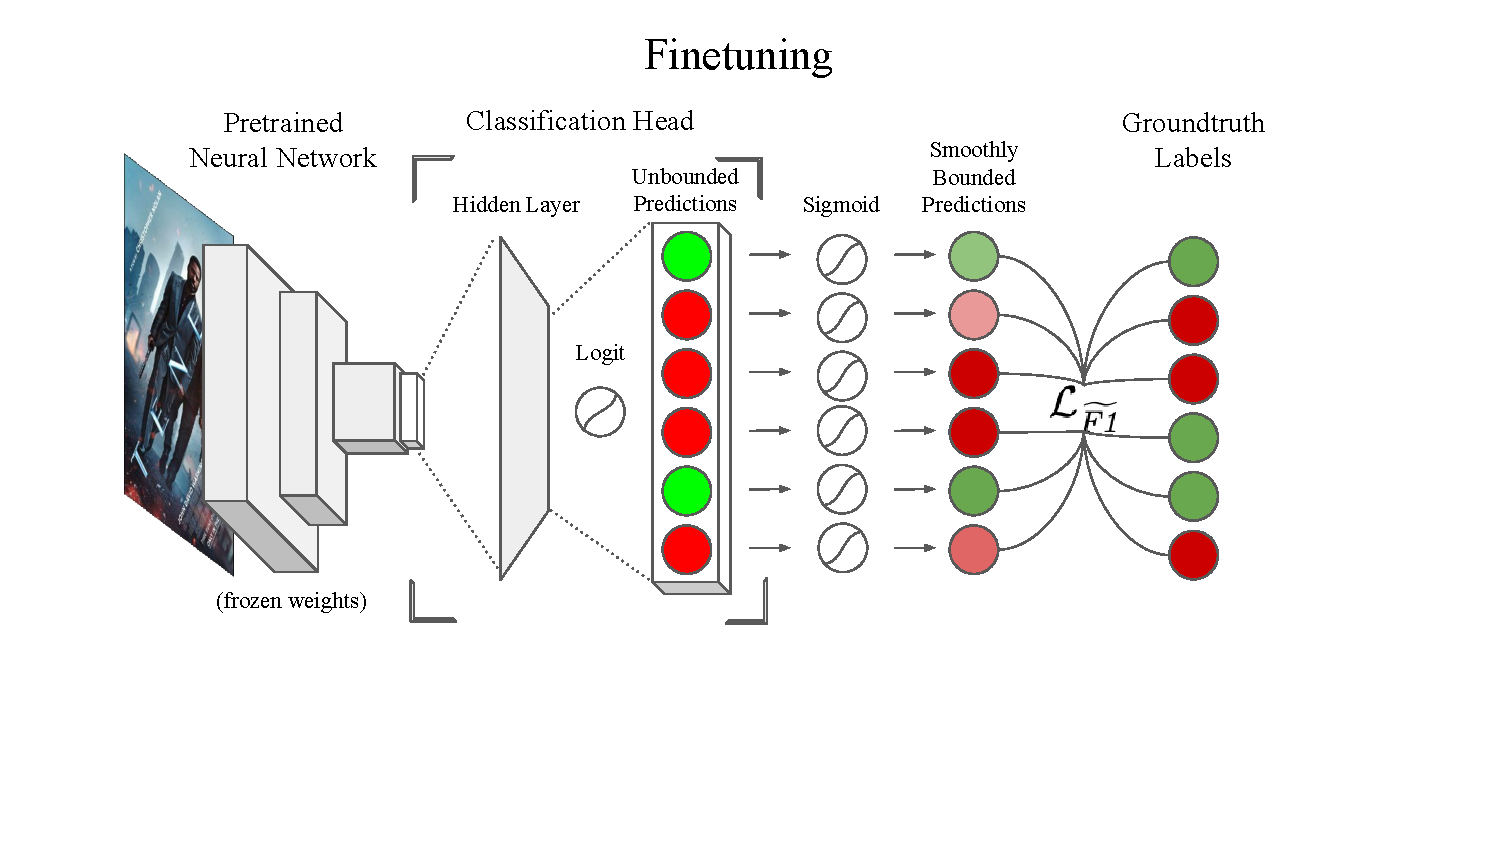
\includegraphics[page=1,width=\linewidth,trim=80 100 110 0,clip]{images/SIGIR2021 Loss Diagram.pdf}
         \caption{Finetuning of a pretrained neural network with an adapted classification head and using sigmoidF1 as a loss function..}
     \end{subfigure}
     \hspace{.02\linewidth}
     \begin{subfigure}{0.36\linewidth}
         \centering
         \includegraphics[page=2,width=\linewidth,trim=190 100 210 0,clip]{images/SIGIR2021 Loss Diagram.pdf}
         \caption{During inference, unbounded predictions are transformed to predictions with a Softmax.}
     \end{subfigure}
     \vspace{.5\baselineskip}
\caption{Learning framework used in the CoMMaL framework and specifically for sigmoidF1 as a loss function.}
\label{fig:architecture}
\end{figure*}

Since the focus of this paper is in comparing loss functions and not neural network architectures, we chose efficient network architectures in terms of accuracy and computation.
For the moviePoster image dataset, we use a MobileNetV2~\cite{mobileNet} architecture that was pretrained on ImageNet~\cite{imagenet}. This network architecture is typically used for inference on small computing devices (e.g., smartphones). We use a version of MobileNetV2 already stripped off of its original classification head.\footnote{The pretrained network can be loaded here \url{https://tfhub.dev/google/imagenet/mobilenet_v2_100_224/feature_vector/4}.}
For the three text datasets, we use DistilBert~\cite{distilBert} as implemented in Hugging Face. This is a particularly efficient instance of the BERT model.\footnote{The pretrained network can be loaded here \url{https://huggingface.co/transformers/model_doc/distilbert.html}.}.
In both cases, we use the final pretrained layer as an embedding of the input. In order to make sure that the results of different loss functions are comparable, we fix the model weights of the pretrained MobileNetV2 and DistilBert and keep the hyperparameter values that were used to train them from scratch. We also initialize the model weights with the same TensorFlow internal random seeds across training sessions.

A similar classification head is used for both MobileNetV2 and DistilBert. It consists of a latent representation layer (the final pretrained layer mentioned above) connected with a RELU activation. This layer is linked to a final classification layer with a linear activation. The dimension of the final layer is equal to the number of classes in the dataset. When computing focalLoss and crossEntropy, a softmax transformation transforms the unbounded last layer to a $[0,1]$ bounded vector. When computing sigmoidF1 loss, a sigmoid transformation is operated instead, which results in a sparser $[0,1]$ vector. At inference time, the last layer is used for prediction and is bounded with a softmax function. A threshold must then be chosen at evaluation time to compute different metrics. Figure \ref{fig:architecture} depicts this learning framework. Thresholding regimes at inference time are further discussed in Sections~\ref{sec:evalMetrics} and~\ref{subsec:thresh}.

% \gab{ev. remove losses compared}
% \subsection{Losses Compared}
% \label{section:losssescompared}

% We benchmark sigmoidF1 against three other losses. The cross-entropy loss and its variant for sparse datasets, focal loss, are representatives of the fit-data-to-algorithm approach as they are binary classifiers. The third loss function is unboundedF1 and represents a first step towards CoMMaL.
 
\subsection{Evaluation metrics}
\label{sec:evalMetrics}

In our experimental evaluation, we consider a suite of metrics that are commonly used in the evaluation of multilabel classification to measure the effectiveness of multilabel prediction. Such metrics are based on the confusion matrix tjat we detailed in Section~\ref{section:method} and for which we provided smoothed surrogates to optimize directly.

When true positives and false positives are used, recall that \(t p=\sum_{i \in Y^{+}} \mathds{1}_{\mathbf{p_i} \geq t}\) and \(f p=\sum_{i \in Y^{-}} \mathds{1}_{\mathbf{p_i} \geq t}\), and thus a threshold \(t\) must be set. Information on thresholding at inference time is generally hard to find in the recent literature, we thus decide on neutral thresholds before training. For arXiv2020 and moviePosters, we set \(t = 0.5\), as is commonly done in the early literature~\cite{multilabelReview, thresh0.5}.
For the two medical datasets, cancerHallmarks and chemicalExposure, we saw after a few preparatory training rounds that only sigmoidF1 had non-zero results for \(t = 0.5\). Information is a lot more sparse for these dataset, we thus set the evaluation metrics threshold to a reasonable value of $0.05$ and train for $500$ epochs until reaching convergence. 

Extending \(F_1\) to multi-class binary classification amounts to deciding wether or not to pool classes.
In a first pooled iteration, macro \(F_1\)~\cite{multilabelMetrics} equates to creating a single 2x2 confusion matrix for all classes:
%
\begin{equation}
F_1^{macro} = \frac{\sum^c tp_j}{2 \sum^c tp_j + \sum^c fn_j + \sum^c fp_j},
\end{equation}
%
with $\sum^c (\cdot)$ as a short form of $\sum_{j=1}^c(\cdot)$, when summing over each class up to the $c$'th class.
Micro \(F_1\) \cite{threshForF1, multilabelMetrics} amounts to creating one confusion matrix per class or unpooling:
%
\begin{equation}
F_1^{micro} =  \frac{1}{c} \sum_{j=1}^c \frac{tp_j}{2 tp_j + fn_j + fp_j} =  \frac{1}{c} \sum_{j=1}^c F_1^j.
\end{equation}
%
Weighted micro \(F_1\)~\cite{weightedMetrics} is similar but includes weighing to account for class imbalance, i.e., weighing each class by the number of ground-truth positives:
%
\begin{equation}
F_1^{weighted} = \frac{1}{c} \sum_{j=1}^c p_j F_1^j \quad \text{, where } p_j = \sum_i \mathds{1}_{\mathbf{y_i^j} = 1}.
\end{equation}
%
We also define micro precision% and micro recall
%
\begin{equation}
\begin{aligned} P^{micro} &=  \frac{1}{c} \sum_{j=1}^c \frac{tp_j}{tp_j+fp_j}% \\ R^{micro} &=  \frac{1}{c} \sum_{j=1}^c \frac{tp_j}{tp_j+fn_j}
\end{aligned}
\end{equation}
%
In our experiments, we report on weightedF1, microF1, macroF1, Precision% and Recall
. Macro scores do not differentiate multiclass unilabel classification from multiclass multilabel classification. Micro scores treat classes separately. The \emph{weighted} micro F1 score is a further refinement where class scores are weighted by their representation in the dataset. We thus focus our discussion of experimental results around weightedF1 as we consider this to be the most representative for success on FIMPUL problems. 

There is an interaction between our optimization on sigmoidF1 and our evaluation using (weighted) F1 metrics. If our approach of optimizing for an F1 surrogate succeeds, we expect higher values on F1-related metrics during evaluation. For this reason, we consider and discuss not a single, but multiple metrics.

\subsection{Hyperparameters and reproducibility}
\label{subsec:hypers}

We choose to ignore classes that are underrepresented, in order to give the model a fair chance at learning from at least a few examples. We define underrepresentation as a global irrelevance threshold $b$ for classes: any class $c$ that is represented less than $b$ times is considered irrelevant. We decided to set an irrelevance threshold $b$ on all datasets prior to conducting experiments, so as to not finetune for that feature. It was set to 1000 for both \emph{arXiv2020} (145 of the original 155 classes remaining) and \emph{moviePosters} (14 of the 28 classes remaining) and at 10 for \emph{chemicalExposure} (all 38 classes remaining) and \emph{cancerHallmarks} (all 33 classes remaining), in proportion to the number of classes and labels in each dataset. The sensitivity study below illustrates what happens when we let $t$ vary over the arXiv2020 dataset.

Batch size is set at a high value of 256. We thus increase accuracy over traditional losses~\cite{bigBS}, but also allow heterogeneity in the examples within the batch, thus collecting enough values in each quadrant of the confusion matrix (see Section \ref{sec:orgc5d29d7} for a discussion on batch sizes).

Regarding the sigmoidF1 hyperparameters $\beta$ and $\eta$, we performed a grid search with the values in the range $[1,30]$ for $\beta$ and $[0, 2]$ for $\eta$.
In our experiments, we evaluate the sensitivity of our method to these hyperparameters (see Figure~\ref{fig:sigmoid}).

We made sure to split the data in the same training, validation and test sets for each loss function. Our code, dataset splits and other settings are shared to ensure reproducibility of our results. 

We performed our experiments on Amazon Web Services cloud machines with parallelization on up to 16 GPUs \textit{p2.16xlarge}, with TensorFlow 2 as a gradient-descent backend.
